\documentclass[14pt, a4paper]{extarticle}
\usepackage{GOST}
\usepackage{array}
\usepackage{verbatim}
\usepackage[detect-all]{siunitx}
\usepackage{amsmath}
\usepackage{amssymb}
\usepackage[utf8]{inputenc}
\usepackage{hyperref}
\usepackage{tempora}

\makeatletter
\renewcommand\@biblabel[1]{#1.}
\makeatother

\usepackage{listings}
\lstset{ 
	language=C,
	basicstyle=\small, 
	numbers=left, 
	numberstyle=\tiny,
	stepnumber=1,
	numbersep=5pt,
	showspaces=false,            
	showstringspaces=false,      
	showtabs=false,             
	frame=single,            % рисовать рамку вокруг кода
	tabsize=4,      
	commentstyle=\color{green},
	keywordstyle=\color{blue}\textbf,
	numberstyle=\scriptsize\color{gray}, % the style that is used for the line-numbers
	rulecolor=\color{black},
	captionpos=t,
	breaklines=true,         % автоматически переносить строки 
	breakatwhitespace=false, % переносить строки по пробелу
	%escapeinside={\#*}{*)} 
}


\usepackage{pgfplots}
\usepackage{filecontents}
\usetikzlibrary{datavisualization}
\usetikzlibrary{datavisualization.formats.functions}

\begin{document}
	
\begin{table}[ht]
	\centering
	\begin{tabular}{|c|p{400pt}|} 
		\hline
		\begin{tabular}[c]{@{}c@{}} 
\includegraphics[scale=1]{source/b_logo.jpg} \\\end{tabular} &
		\footnotesize\begin{tabular}[c]{@{}c@{}}\textbf{Министерство~науки~и~высшего~образования~Российской~Федерации}\\\textbf{Федеральное~государственное~бюджетное~образовательное~учреждение}\\\textbf{~высшего~образования}\\\textbf{«Московский~государственный~технический~университет}\\\textbf{имени~Н.Э.~Баумана}\\\textbf{(национальный~исследовательский~университет)»}\\\textbf{(МГТУ~им.~Н.Э.~Баумана)}\\\end{tabular}  \\
		\hline
	\end{tabular}
\end{table}
\noindent\rule{\textwidth}{4pt}
\noindent\rule[14pt]{\textwidth}{1pt}
\hfill 
\noindent
\makebox{ФАКУЛЬТЕТ~}%
\makebox[\textwidth][l]{\underline{~«Информатика и системы управления»~~~~~~~~~~~~~~~~~~~~~~~~~~~~~~~~~}}%
\\
\noindent
\makebox{КАФЕДРА~}%
\makebox[\textwidth][l]{\underline{~«Программное обеспечение ЭВМ и информационные технологии»~}}%
\\

\begin{center}
	\vspace{1.5cm}
	{\bf\huge Отчёт\par}
	{\bf\Large по лабораторной работе № 5\par}
	\vspace{0.7cm}
\end{center}


\noindent
\makebox{\large{\bf Название:}~~~}
\makebox[\textwidth][l]{\large\underline{~Буферизованный и не буферизованный ввод-вывод~}}\\


\noindent
\makebox{\large{\bf Дисциплина:}~~~}
\makebox[\textwidth][l]{\large\underline{~Операционные системы~~~~~~~~~~~~~~~~~~~~~~~~~~}}\\

\vspace{1.5cm}
\noindent
\begin{tabular}{l c c c c c}
	Студент      & ~ИУ7-65Б~               & \hspace{2.5cm} & \hspace{2cm}                 & &  Д.О. Склифасовский \\\cline{2-2}\cline{4-4} \cline{6-6} 
	\hspace{3cm} & {\footnotesize(Группа)} &                & {\footnotesize(Подпись, дата)} & & {\footnotesize(И.О. Фамилия)}
\end{tabular}

\noindent
\begin{tabular}{l c c c c}
	Преподаватель & \hspace{5cm}   & \hspace{2cm}                 & & ~~~~~~Н.Ю. Рязанова~~~~~~\\\cline{3-3} \cline{5-5} 
	\hspace{3cm}  &                & {\footnotesize(Подпись, дата)} & & {\footnotesize(И.О. Фамилия)}
\end{tabular}

\vspace{0.6cm}
\begin{center}	
	\vfill
	\large \textit {Москва, 2021}
\end{center}

\thispagestyle {empty}
\pagebreak

\clearpage
\section*{Программа 1}
\begin{lstlisting}
#include <stdio.h>
#include <fcntl.h>

int main()
{
	int fd = open("alphabet.txt", O_RDONLY);
	
	FILE *fs1 = fdopen(fd, "r");
	char buff1[20];
	setvbuf(fs1, buff1, _IOFBF, 20);
	
	FILE *fs2 = fdopen(fd, "r");
	char buff2[20];
	setvbuf(fs2, buff2, _IOFBF, 20);
	
	int flag1 = 1, flag2 = 2;
	while (flag1 == 1 || flag2 == 1)
	{
		char c;
		flag1 = fscanf(fs1, "%c", &c);
		if (flag1 == 1)
		{
			fprintf(stdout, "%c", c);
		}
		flag2 = fscanf(fs2, "%c", &c);
		if (flag2 == 1)
		{
			fprintf(stdout, "%c", c);
		}
	}
	return 0;
}
\end{lstlisting}
\begin{figure}[h!]
	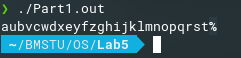
\includegraphics[scale=1]{source/Part1.png}
\end{figure}
С помощью системного вызова open() создается дескриптор открытого на чтение файла. Системный вызов open() возвращает индекс в массиве fd структуры files\_struct.\\
fdopen() создает структуру типа FILE, которая ссылается на дескриптор, созданный системным вызовом open.\\
Система создаст буфер на 20 байт. \\
Вызов setvbuf свяжет поток, ссылающийся на открытый файл, с созданным буфером. Параметр \_IOFBF указывает на режим полной буферизации.\\
Далее в цикле выполняется fscanf() поочерёдно для fs1 и fs2. Так как установлена полная буферизация, то при первом вызове fscanf() буфер будет заполнен полностью либо вплоть до конца файла, а f\_pos установится на следующий за последним записанным в буфер символ.\\
Результатом является строка "Aubvcwdxeyfzghijklmnopqrst"\\

\begin{figure}[h!]
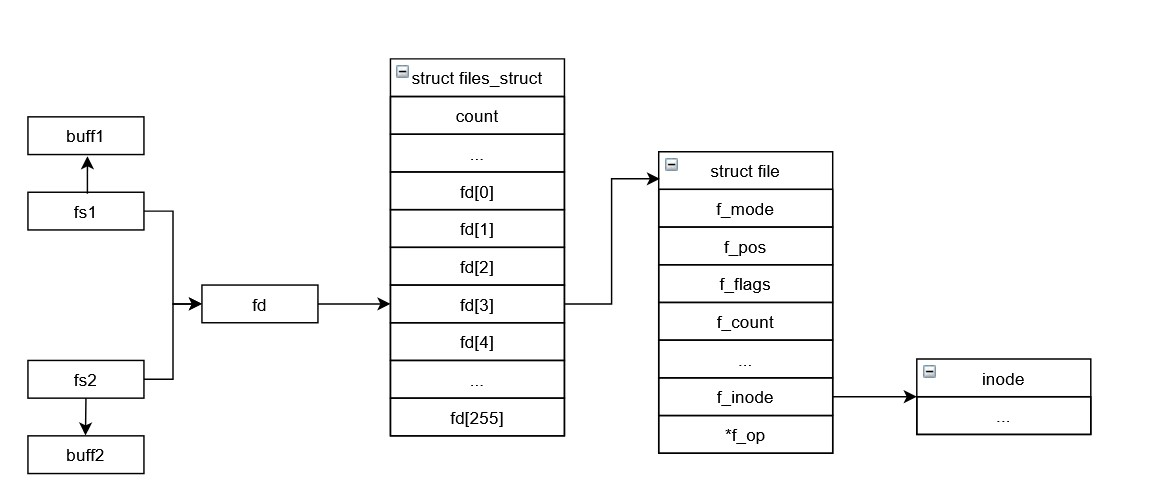
\includegraphics[scale=0.6]{source/diag1.jpg}
\end{figure}
\clearpage
\section*{Программа 2}
\begin{lstlisting}
#include <fcntl.h>

int main()
{
	char c;
	
	int fd1 = open("alphabet.txt", O_RDONLY);
	int fd2 = open("alphabet.txt", O_RDONLY);
	
	while (read(fd1, &c, 1) == 1 && read(fd2, &c, 1) == 1)
	{
		write(1, &c, 1);
		write(1, &c, 1);
	}
	return 0;
}
\end{lstlisting}
\begin{figure}[h!]
	
\includegraphics[scale=1]{source/Part2.png}
\end{figure}
При вызове системного вызова open() создается дескриптор файла в системной таблице файлов, открытых процессом и запись в системной таблице открытых файлов. \\
файл открывается 2 раза, поэтому в таблице открытых файлов будет 2 дескриптора и каждый такой дескриптор имеет собственный f\_pos.\\
В цикле выполнятся read(), считывающий символ и write(), записывающий символ в стандартный поток. Указатель f\_pos изменяется независимо от другого дескриптора.
\begin{figure}[h!]
	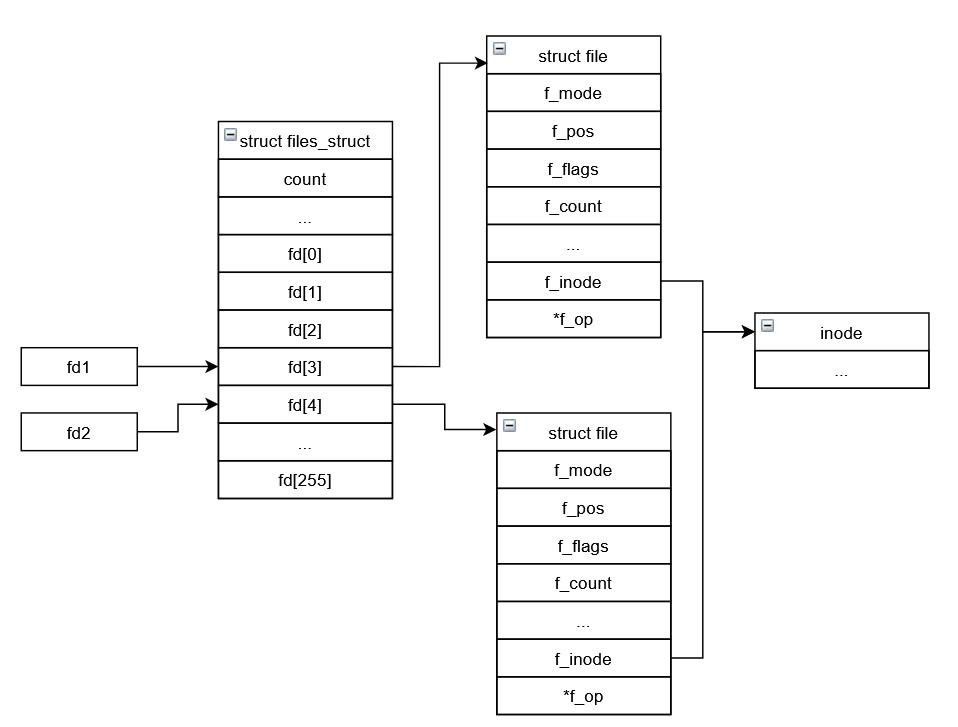
\includegraphics[scale=0.60]{source/diag2.jpg}
\end{figure}
\newpage
\section*{Программа 2 с потоками}
\begin{lstlisting}
#include <fcntl.h>
#include <pthread.h>
#include <stdio.h>
#include <stdlib.h>

void *read_file(int *fd)
{
	char c;
	while (read(*fd, &c, 1) == 1)
	{
		write(1, &c, 1);
	}
	return 0;
}

int main()
{    
	int fd1 = open("alphabet.txt", O_RDONLY);
	int fd2 = open("alphabet.txt", O_RDONLY);
	
	pthread_t thread1, thread2;
	
	int stat1 = pthread_create(&thread1, NULL, read_file, &fd1);
	if (stat1 != 0)
	{
		printf("Cannot create thread 1\n");
		return -1;
	}
	
	int stat2 = pthread_create(&thread2, NULL, read_file, &fd2);
	if (stat2 != 0)
	{
		printf("Cannot create thread 2\n");
		return -1;
	}
	
	pthread_join(thread1, NULL);
	pthread_join(thread2, NULL);
	
	return 0;
}
\end{lstlisting}
\begin{figure}[h!]
	
\includegraphics[scale=1]{source/Part2Thread.png}
\end{figure}
В данном случае потоки читают один и тот же файл параллельно, каждый поток выполнит запись независимо, что приведет к повтору каждого символа.
\newpage
\section*{Программа 3}
\begin{lstlisting}
#include <stdio.h>
#include <sys/stat.h>

int main()
{
	struct stat bufStat;
	
	FILE *file1 = fopen("result.txt", "w");
	stat("result.txt", &bufStat);
	printf("First opening\n\tinode\t= %ld\n\tsize\t= %ld\n", bufStat.st_ino, bufStat.st_size);
	
	FILE *file2 = fopen("result.txt", "w");
	stat("result.txt", &bufStat);
	printf("Second opening\n\tinode\t= %ld\n\tsize\t= %ld\n", bufStat.st_ino, bufStat.st_size);
	
	char needChar = 'a';
	while (needChar <= 'z') 
	{
		if (needChar % 2 == 0)
		{
			fprintf(file1, "%c", needChar);
		}
		else
		{
			fprintf(file2, "%c", needChar);
		}
		needChar++;
	}
	
	fclose(file1);
	stat("result.txt", &bufStat);
	printf("First closing\n\tinode\t= %ld\n\tsize\t= %ld\n", bufStat.st_ino, bufStat.st_size);
	
	fclose(file2);
	stat("result.txt", &bufStat);
	printf("Second closing\n\tinode\t= %ld\n\tsize\t= %ld\n", bufStat.st_ino, bufStat.st_size);
	
	return 0;
}
\end{lstlisting}
\begin{figure}[h!]
	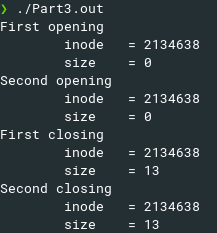
\includegraphics[scale=1]{source/Part3.png}
\end{figure}
Файл открывается 2 раза для записи. Создается два дескриптора открытых файлов, следовательно, два независимых f\_pos. Но они ссылаются на один inode.\\
fopen и fprintf функции stdio – библиотеки буферизуемого ввода/вывода, поэтому сначала информация пишется в буфер. \\
В  икле происходит запись каждого четного символа в буфер, соответсвующий file1 и каждого нечетного в буфер, соответсвующий file2. Запись в файл из буфера происходит при вызове функции fclose().\\
При вызове fclose() для file1 буфер записывается в файл.\\
При вызове fclose() для file2, все содержимое файла перезаписывается содержимым буфера для file2.\\ 
В итоге, данные из первого буфера будут утеряны.
\begin{figure}[h!]
	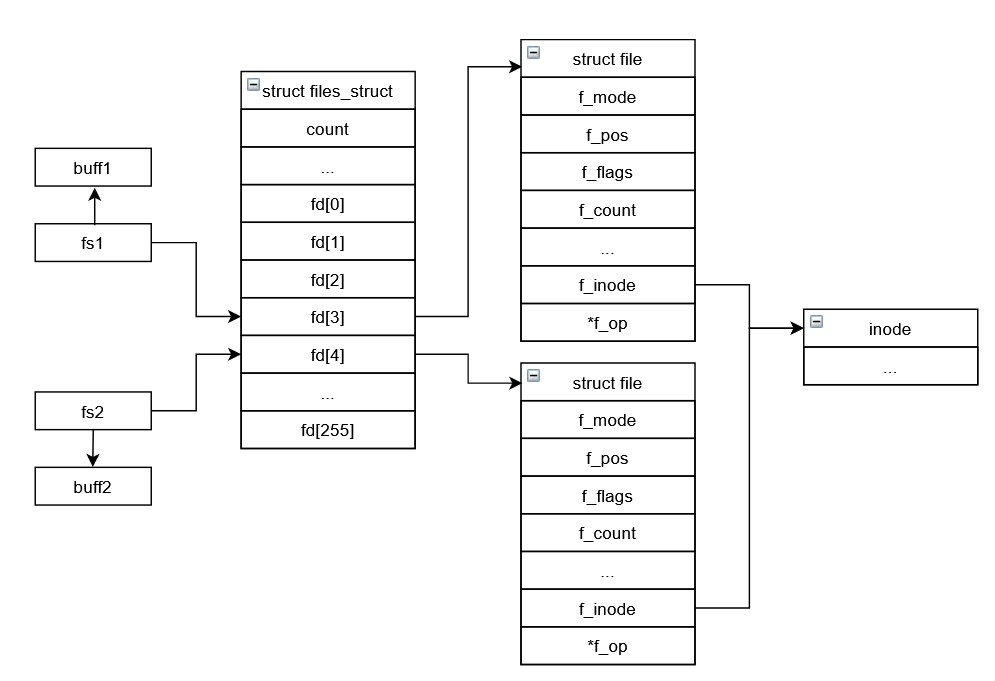
\includegraphics[scale=0.60]{source/diag3.jpg}
\end{figure}
\newpage
\section*{Программ 3 с потоками}
\begin{lstlisting}
#include<stdio.h>
#include<stdlib.h>
#include<sys/stat.h>
#include<pthread.h>

void *write(int *fd)
{
	struct stat bufStat;
	
	FILE *file = fopen("result.txt", "w");
	stat("result.txt", &bufStat);
	printf("Opening file\n\tinode\t= %ld\n\tsize\t= %ld\n", bufStat.st_ino, bufStat.st_size);
	
	char needChar = 'a' + *fd - 1;    
	while (needChar <= 'z') 
	{
		fprintf(file, "%c", needChar);
		needChar += 2;
	}
	
	fclose(file);
	stat("result.txt", &bufStat);
	printf("Closing\n\tinode\t= %ld\n\tsize\t= %ld\n", bufStat.st_ino, bufStat.st_size);
}

int main()
{
	pthread_t thread1, thread2;
	int fd1 = 1,
	fd2 = 2;
	
	int stat1 = pthread_create(&thread1, NULL, write, &fd1);
	if (stat1 != 0)
	{
		printf("Cannot create thread 1\n");
		return -1;
	}
	
	int stat2 = pthread_create(&thread2, NULL, write, &fd2);
	if (stat2 != 0)
	{
		printf("Cannot create thread 2\n");
		return -1;
	}
	
	pthread_join(thread1, NULL);
	pthread_join(thread2, NULL);
	return 0;
}
\end{lstlisting}
\begin{figure}[h!]
	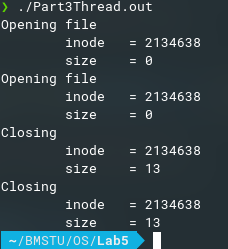
\includegraphics[scale=1]{source/Part3Thread.png}
\end{figure}
В данном случае потоки записывают символ в соответствующий буфер. В результате вызова fclose, в файле сохранится содержимое буфера, чей поток завершится последним.\\



\noindent struct stat \{\\
\indent dev\_t st\_dev; /* устройство */ \\
\indent ino\_t st\_ino; /* inode */\\
\indent mode\_t st\_mode; /* режим доступа */\\
\indent nlink\_t st\_nlink; /* количество жестких ссылок */\\
\indent uid\_t st\_uid; /* идентификатор пользователя-владельца */\\
\indent gid\_t st\_gid; /* идентификатор группы-владельца */\\
\indent dev\_t st\_rdev; /* тип устройства */\\
\indent /* (если это устройство) */\\
\indent off\_t st\_size; /* общий размер в байтах */\\
\indent blksize\_t st\_blksize; /* размер блока ввода-вывода */\\
\indent /* в файловой системе */\\
\indent blkcnt\_t st\_blocks; /* количество выделенных блоков */\\
\indent time\_t st\_atime; /* время последнего доступа */\\
\indent time\_t st\_mtime; /* время последней модификации */\\
\indent time\_t st\_ctime; /* время последнего изменения */\\
\};\\
typedef struct \_\_sFILE \{\\
\indent …\\
\indent unsigned char *\_p;\\
\indent short \_flags;\\
\indent short \_file;\\
\indent struct \_\_sbuf \_bf;\\
\indent …\\
\indent void *\_cookie;\\
\indent …\\
\indent struct \_\_sbuf \_ub;\\
\indent struct \_\_sFILEX *\_extra;\\
\indent int \_ur;\\
\indent …\\
\indent unsigned char \_ubuf[3];\\
\indent unsigned char \_nbuf[1];\\
\indent …\\
\indent struct \_\_sbuf \_lb;\\
\indent int \_blksize;\\
\indent fpos\_t\_offset;\\
\} FILE;\\



\end{document}